%%%%%%%%%%%%%%%%%%%%%%%%%%%%%%%%%%%%%%%%%%%%%%%%%%%%%%%%%%%%%%%%%%%%%%%%%%%%%
\section{GPGPU Introduction}

GPGPU (\textit{General Purpose computation on Graphics Processor Unit}), also known as \textit{GPU Computing}, is the utilization of the graphic adapter of a personal computer to perform generic and non-graphic related computation usually handled by the CPU.\\
Once designed and optimized specifically to perform only fixed graphic calculations, modern GPUs are evolving into \emph{high-performances many-core} processors that can be virtually used to perform any task. Developers who port their applications to GPUs are able to achieve speedups of orders of magnitude vs. optimized CPU implementations.\cite{GPGPUORG:About}\\
The reason why GPUs are so fast has to be searched in the nature of what graphic rendering is about: an \emph{intensive parallel computetion} and , for this reason, GPUs are engineered to work specifically on \emph{data processing}, rather than data caching and flow control like CPUs. (\textbf{Figure \ref{fig:cpuvsgpu_scheme}})

\begin{figurehere}
 \centering
 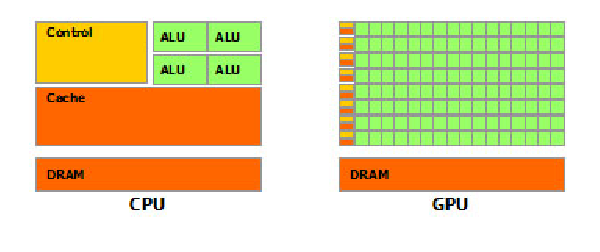
\includegraphics[width=8cm, height=4cm]{./eps/GPU_CPU_struct.eps}
 \caption{GPUs are more focused to computation rather than data caching.}
 \label{fig:cpuvsgpu_scheme}
\end{figurehere}

Moreover, computational units of GPUs are specialized to perform simple operation but \emph{in parallel}.\\
GPUs have been built to exploit application parallelism, and a single graphic adapter can host hundreds, if not thousands, of cores; this translates in TeraFlops of operations per second compared to the "`few"' GigaFlops a CPU can handle alone. (\textbf{Figure \ref{fig:cpuvsgpu}})

\begin{figurehere}
 \centering
 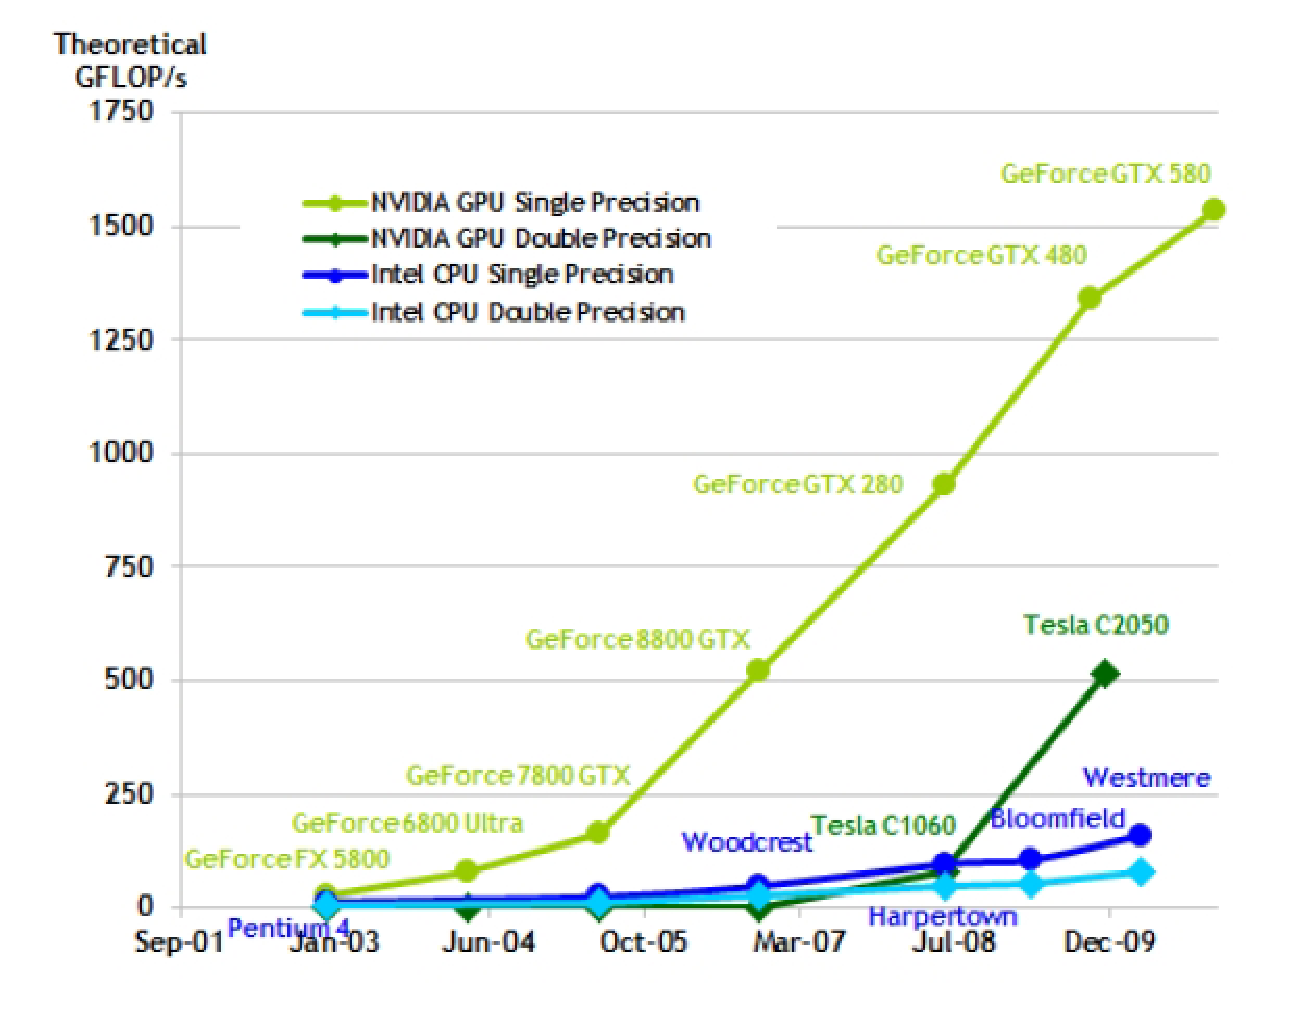
\includegraphics[width=8cm, height=4cm]{./eps/GPU_CPU_chart.eps}
 \caption{CPU vs GPU growth rate.}
 \label{fig:cpuvsgpu}
\end{figurehere}

Due to its parallel nature, GPU computing can be very effective for applications involving huge amount of data, especially if the data can be structured in structures like vectors and arrays.
Parallel GPU computation can be applied in various applications and research-field, from computer vision, to mathematical simulations, to bio-informatics, and it often allows to achieve in a few months the same results that would have required years to achieve with a standard CPU-only approach (with speedups of the order of 250x,350x).

\begin{figurehere}
 \centering
 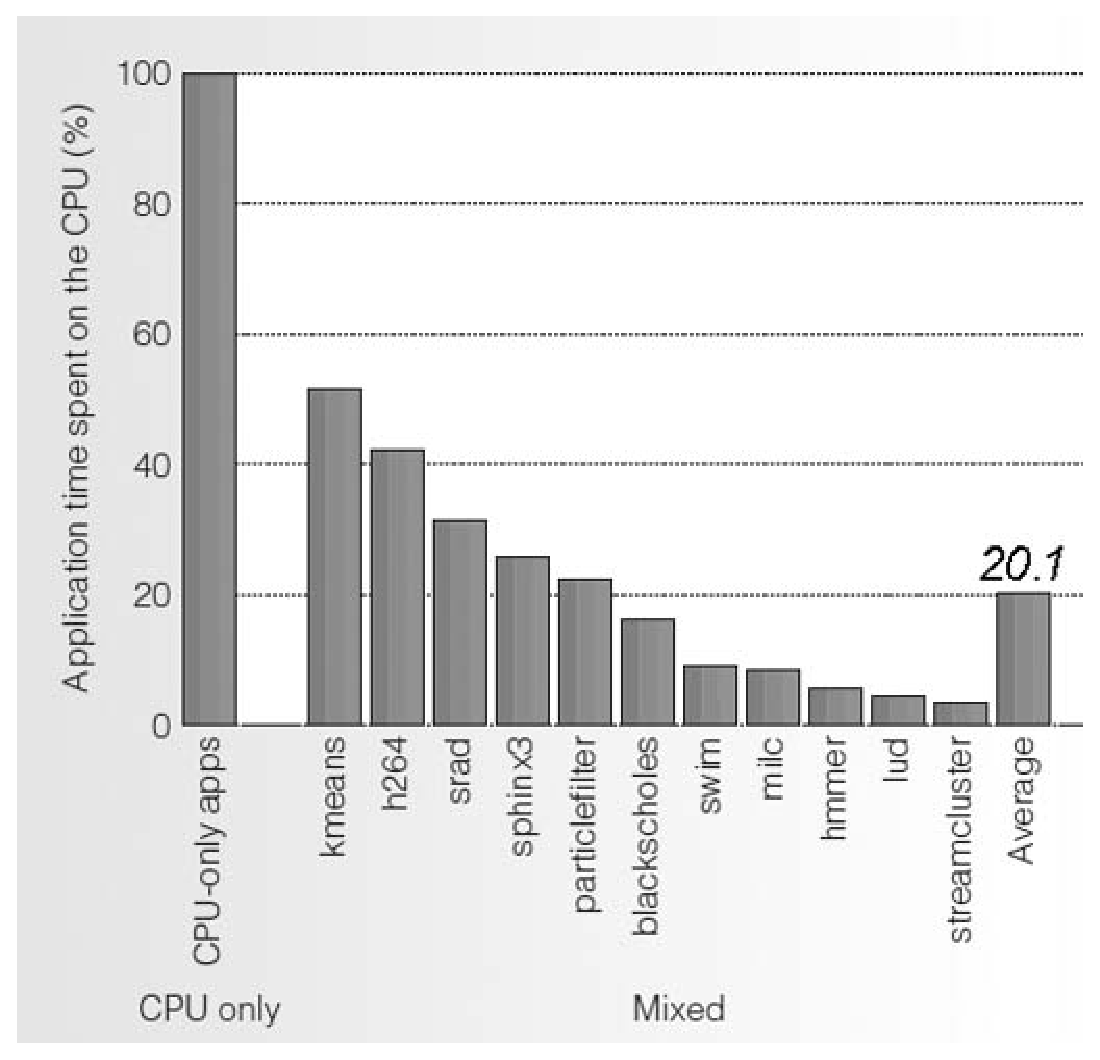
\includegraphics[width=6cm, height=4cm]{./eps/CPU_usage.eps}
 \caption{Time spent on the CPU on various benchmarks using mixed CPU-GPU computation. \cite{Arora:12:Redefining}}
 \label{fig:cpuload}
\end{figurehere}


As you can see in \textbf{Figure \ref{fig:cpuload}}, GPU can offload the CPU from most of its work, but this doesn't mean that CPU performance is no longer critical. Many applications don't (and can't) map all their code to the GPU, and in certain cases the CPU can run some part of the code more effectively than the GPU.
Furthermore, not all the code can be mapped easily and clearly on the GPU, as programming in this way can be way more difficult than programming in a standard way, it is not possible to simply "`port"' the code from the CPU to the GPU.

%-----------------------------------------------------------------------------
\subsection{Basic Principles} \label{sect:principles}
% Please avoid separations in titles
% and separate text manually

In this section we'll introduce some of the basic principles behind GPGPU programming. Some of these concepts are directly related to the "`graphical-oriented"' way in which the GPU operates, and having a little kwowledge of basic concepts of computer gprahics can help to understand why GPU computing is so fast. For instance, GPUs can handle bidimensional matrices natively because that's the natural way to represent images in memory, while CPUs are limited to always work on single dimension arrays.\\
A GPU is basically a \textit{stream processor}\footnote{Stream Processing refers to a SIMD (Single Instruction Multiple Data) paradigm that allows application to exploit (limited) parallel processing over data.}: a single \textbf{kernel} is executed over a stream of data in a monolitic fashion.
Thanks to the GPU architecture, the data can be elaborated in parallel, and more than one kernel can be executed at the same time.

\subsubsection{Textures = Arrays}
Due to the linear structure of memory, traditional CPUs cannot \emph{physically} create multi-dimensional array, and accessing single rows and columns of a matrix is achieved by offsetting memory addresses of a large linear array. Each one of these "`jump"' in memory translates directly in performance loss.\\
On the other hand, GPUs are architectured to work natively with textures, that are naturally represented in memory by two-dimensional arrays.\\
The ability to work directly over bidimensional (and three-dimensional) memory structures is one of the main reason why GPUs are much more faster than CPUs when it comes to elaborate data.\\
Besides, CPUs can handle memory structures much more bigger (and virtually infinite) compared to the those available for the GPU, as many graphic adapters can only work on textures limited in size. The usual maximum size of a texture is usually 2048*2048, or 4096*4096, but modern can reach sizes of 8192*8192.
The maximum texture size available for a certain graphic adapter can usually be easily retrieved by simple queries made available by the programming API you are using.

\begin{CLCode}
For Example, with OpenCL, you can obtain the maximum supported texture size with the \textsl{clGetDeviceInfo()} function, passing the
\textsl{CL\_DEVICE\_IMAGE2D\_MAX\_WIDTH} and \textsl{CL\_DEVICE\_IMAGE2D\_MAX\_HEIGHT} as parameters.
\end{CLCode}

We will discuss how textures (and \textit{memory objects} in general) are created and accessed in Section \ref{sect:openCLArch}, when we will introduce the OpenCL API.

\subsubsection{Kernels}
If you are familiar with graphic pipeline programming, kernels are the GPGPU equivalent of \textbf{shaders}.\\
Kernel programming is the core concept of the GPU computation and forces the developer to think in a different way as he is used to, as kernels are oriented toward \emph{parallel execution over stream of data}, while ``standard'' CPU programming is oriented toward a classical \emph{loop-iterated} implementation.\\
Since the data of our applicationis stored into multi-dimensional memory objects (the equivalent of a graphical texture), GPU computing basically consists in feeding this memory structures to a kernel that will execute its code over different data elements simultaneously, like a GPU shader apply the same transformation on multiple pixels at the same time to obtain a new image.\\
The output of kernel computation will be a new memory object that contains the result of the calculation. If we keep in mind that GPUs were born to elaborate graphics data, it will be easier to understand how kernels work and the best approach to be taken when it comes to write a GPGPU application.
To understand how this mechanism works, here's an example of a simple graphical shader written in HLSL language that basically scans a texture to find black pixels and turn them to white:

{\footnotesize\begin{verbatim}
float3 BlackToWhite(PixelShaderInput input)
{
  if(input.Color.r == 0 &&
	     input.Color.g == 0 && 
     input.Color.b == 0)
     return float3(1,1,1);
  else
     return input.Color;
}
\end{verbatim}}

The same code in a traditional loop-oriented implementation will be something like:

{\footnotesize\begin{verbatim}
void BlackToWhite(float input[4096][4096][3],
                  float output* [4096][4096][3])
{
  for	(int y=0,y<4096,y++)
    for(int x=0;x<4096;x++)
    {
      if(input[x][y][0] == 0 &&
         input[x][y][1] == 0 &&
         input[x][y][2] == 0)
      {
         *output[x][y][0] = 1;
         *output[x][y][1] = 1;
         *output[x][y][2] = 1;
      }
      else
      {
         *output[x][y][0] = input[x][y][0];
         *output[x][y][1] = input[x][y][1];
         *output[x][y][2] = input[x][y][2];
      }
    }
}
\end{verbatim}}


By comparing the two examples, we can note two fundamental things:

\begin{enumerate}
	\item In the shader we do not implement any cycle, the code is iterated \emph{automatically} on every element of the input structure. Also there is no mapping between the input and the output, but only a \textbf{single return}, because the output element is automatically mapped to the same texture coordinate of the input.
	\item Since GPU are meant to work with colors, shaders can natively work on 4 different channels at a time (RGBA), making GPU computation even more versatile and powerful.
\end{enumerate}

While shaders have to be written in low-level specific languages like HLSL or GLSL, kernels take advantage of APIs that allow the programmers to implement and execute them like normal functions. We'll discuss how to implement some kernel application in Section \ref{sect:kernelImplementation}.

\begin{CLCode}
For Example, using the OpenCL API, you can create objects of type \textbf{cl\_kernel} and initialize them with the \textbf{clCreateKernel()} function.
\end{CLCode}


\subsubsection{Computation and feedback}
Since GPU's final purpose is to draw something on screen, GPGPU application cannot be simply ``executed'' like traditional ones, and kernels (although they are basically functions) cannot be simply ``called''. To execute a kernel application over the GPU we have to make it think that it is actually drawing something. In GPU computing, ``to execute something'' translates to ``\textit{to draw something}''.
The operations needed for a kernel call (and their shader execution equivalent) are summarized in \textbf{Table \ref{tab:computeVsDraw}}.\\

\begin{tablehere}
{\footnotesize
\begin{tabular}{|p{0,3cm}|p{7cm}|}\hline
~ & \textbf{Drawing perspective}\\ \hline
1) & Assign the input texture to a texture channel of the graphic adapter\\ \hline
2) & Setting the drawing surface \\ \hline
3) & Define the quad to be drawn. The quad must fit the entire viewport and the texture must be mapped to it.\\ \hline
4)� & Load the shader\\ \hline
5) & Render the quad�\\ \hline
~ & ~\\ \hline
~ & \textbf{Computation perspective}\\ \hline
1) & Define the input data and feed it to the kernel\\ \hline
2) & Define the memory object where the output data will be stored\\ \hline
3) & Initialize the indices and setting the bounds of the loop \\ \hline
4) &  ~\\ \hline
5) & Iterate through data and execute the kernel.\\ \hline
\end{tabular}}
  \caption{Drawing and Kernel Execution comparison\\}
	\label{tab:computeVsDraw}
\end{tablehere}

After the drawing (the computation) has been performed, the result is stored in the target surface.

%This is a citation \cite{Norman09Learn} and here is another citation
%\cite{Peyton93Howto}.  Lorem ipsum dolor sit amet, consectetur adipiscing elit.


%And this is the reference to a single column figure (see {\bf Figure
%\ref{fig:myfigure1}}).  Lorem ipsum dolor sit amet, consectetur adipiscing elit.

%\begin{figurehere}
% \centering
% \includegraphics[width=8cm, height=4cm]{./eps/placeholder.eps}
% \caption{Some single-column figure caption.}
% \label{fig:myfigure1}
%\end{figurehere}


%-----------------------------------------------------------------------------
\subsection{GPGPU Programming Languages}

In this section we will briefly introduce the most common languages and APIs to develop GPGPU applications.

\subsubsection{CUDA (www.nvidia.com)} \label{sect:CUDA}
CUDA is the parallel programming platform introduced by Nvidia in 2006 and it has currently reached version 5.
The main focus of CUDA is on \textbf{automatic scalability}: the program model forces the programmer to partition the main problem into coarse sub-problems that can be solved independently in parallel, and these threads are automatically scaled in runtime over the many cores different GPUs may have (\textbf{Figure \ref{fig:scalability}}).

\begin{figurehere}
 \centering
 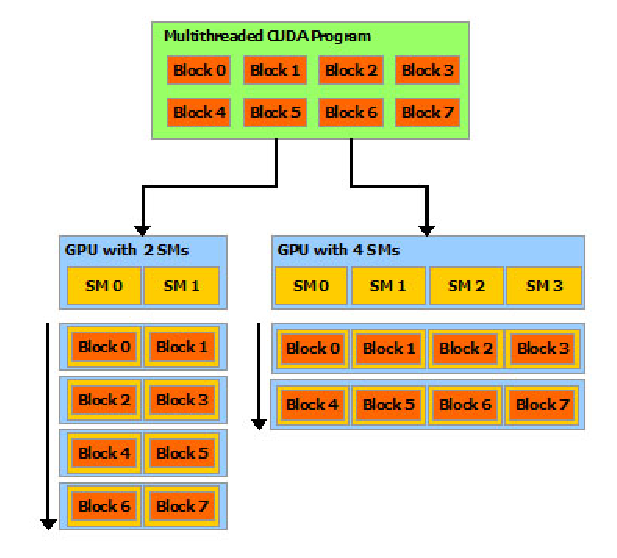
\includegraphics[width=8cm, height=4cm]{./eps/scalability.eps}
 \caption{CUDA executables are automatically scaled over the various SMs (Stream Multiprocessors) a GPU may have : a GPU with more multiprocessors will automatically execute the program in less time than a GPU with fewer multiprocessors.}
 \label{fig:scalability}
\end{figurehere}

CUDA is mainly based on C-language and follow the programming model introduced in Section \ref{sect:principles}, with \textit{Kernels} and introduces new concepts like \textbf{thread hiearchy} (allowing to create \textit{multi-dimensional thread blocks} that can be executed in parallel) and \textbf{memory hierarchy} (for example each thread has its own local memory and can share memory with thread in their own block).\\
On the downside, since it is a proprietary framework, CUDA executables will only run on Nvidia graphic cards, and the code cannot fall back on the CPU in the case a CUDA accelerated hardware is not available on the system.\cite{siroro:GPUComparison}

\subsubsection{OpenCL (www.khronos.org/opencl/)}
OpenCL (Open Computing Language) is the parallel programming model developed by the Khronos group that focuses on cross-platforming: differently from CUDA, OpenCL is supported on a wide range of devices and can also be used on some embedded or mobile devices like Android phones and iPhones.\\
The current version of OpenCL is 1.2 and it was released in 2011.
We will discuss OpenCL more in deep in Section \ref{}.

\subsubsection{DirectCompute}
Also known as Computer Shader (for more info refer to the msdn library: http://msdn.microsoft.com/) is the GPU computing API developed by Microsoft which is part of the DirectX APIs collection starting from version 11.
Since it is part of the DirectX package, DirectCompute uses HLSL shading language and integrates well with applications already written with the DirectX API, however, its compatibility is limited to desktop graphic adapters that supports DX10 or 11 and only for Windows (Vista or later) operating systems.

\begin{figure*}[t]
  \centering
 \includegraphics[width=16cm, height=4cm]{./eps/placeholder.eps}
 \caption{Some wide-figure caption.}
 \label{fig:myfigure2}
\end{figure*}

And this is the reference to a single column figure (see {\bf Figure
\ref{fig:myfigure2}}). Lorem ipsum dolor sit amet, consectetur adipiscing elit.

%%%%%%%%%%%%%%%%%%%%%%%%%%%%%%%%%%%%%%%%%%%%%%%%%%%%%%%%%%%%%%%%%%%%%%%%%%%%%